
\section{Compondo estruturadamente}
\label{sec:compondoestruturadamente}


%%%%%%%%%%%%%%%%%%%%%%%%%%%%%%%%%%%%%%%%%%%%%%%%%%%%%%%%%%%%%%%%%%%%%%%%%%%%%%%%
\subsection{Escolhendo um motivo rítmico}
Na Figura \ref{fig:motivoritmico1}, 
nos  dois  primeiros \hyperref[subsec:compassobinario]{\textbf{compassos binários}} do ritmo,
 se mostra o  \hyperref[sec:Motivo]{\textbf{motivo}} rítmico M. 
O motivo finaliza na parte fraca do tempo fraco do compasso; assim,
para dar um contraste se variou o final de M para obter M', 
também com dois compassos. M' está localizado ao final do ritmo mostrado na Figura \ref{fig:motivoritmico1}. 
M' finaliza na parte forte do tempo fraco, pelo que se obtêm uma maior sensação de conclusão que em M, 
porém menor da que obteríamos si finaliza-se num tempo forte.
\begin{figure}[H]
     \centering
     \href{https://drive.google.com/file/d/1cswgo6-Sjtg_bXyf1Ck3OcJpVPo_KJEq/view?usp=sharing}{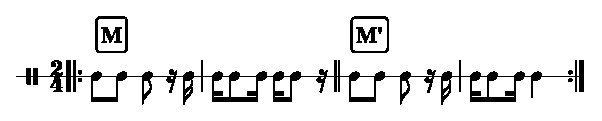
\includegraphics[width=\textwidth]{chapters/cap-musica-topicos/motivo-ritmico-1.eps}}
     \caption{Motivo rítmico MM'.}
     \label{fig:motivoritmico1}
\end{figure}
À concatenação destes dois motivos a chamaremos MM'.


%%%%%%%%%%%%%%%%%%%%%%%%%%%%%%%%%%%%%%%%%%%%%%%%%%%%%%%%%%%%%%%%%%%%%%%%%%%%%%%%
\subsection{Criando a seção A}
\label{subsec:criandoa}
A Figura \ref{fig:section-a} mostra a seção musical A, 
que está composta de duas partes, A1 e A2, 
ambas de 4 \hyperref[subsec:compassobinario]{\textbf{compassos binários}} cada uma, com o mesmo inicio mas com distinto final.
A1 está constituída pelos compassos 1,2,3 e 4; e A2 pelos compassos 1,2,3 e 5.
Ambas partes foram criadas usando como base a frase rítmica de 4 compassos, mostrada na Figura \ref{fig:motivoritmico1}.
     \begin{figure}[H]
	     \centering
	     \href{https://drive.google.com/file/d/1LS2rPtHilL0lv_URBl_Tzs0jZcrSPwgk/view?usp=sharing}{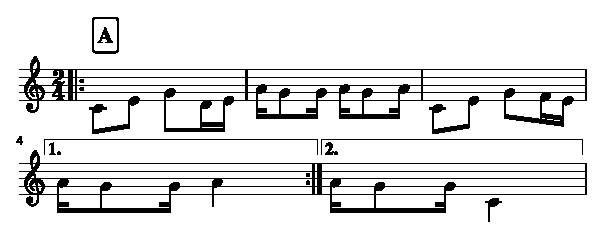
\includegraphics[width=\textwidth]{chapters/cap-musica-topicos/section-a-1.eps}}
	     \caption{Seção musical A.}
	     \label{fig:section-a}
     \end{figure}
É fácil perceber que o compasso 1 é similar ao 3, é que o compasso 2 é similar, ao compasso 5 ou 6; 
as diferencias radicam numa mudança de tons nas últimas notas de 1 e 3, e nas \hyperref[subsec:cadenciamelodica]{\textbf{cadências}} melódicas de 5 e 6, 
onde A1 tem uma \hyperref[subsec:cadenciamelodica]{\textbf{cadência interrompida}} (V-VI) é A2 uma \hyperref[subsec:cadenciamelodica]{\textbf{cadência}} (V-I). 
Seguindo a Tabela \ref{tab:tablefinaltipo} A1 tem um final que deixa uma sensação de algo inconcluso,
e A2 de uma frase suspensiva ou interrogativa.

Com a forma redundante da seção, o único trabalho criativo-mecanico foi achar os tons da melodia nos compassos 1 e 2,
pois os demais compassos são ligeiras variantes.


%%%%%%%%%%%%%%%%%%%%%%%%%%%%%%%%%%%%%%%%%%%%%%%%%%%%%%%%%%%%%%%%%%%%%%%%%%%%%%%%
\subsection{Criando a seção B}
\label{subsec:criandob}
A seção musical B, é criada para ser contrastante com a \hyperref[subsec:criandoa]{\textbf{seção A}},
tentando ser mais alegre;
com este fim, algumas notas \Acht~ foram transformadas em \Sech \Sech;
além disso o compasso 1 foi modificado para iniciar mais alegremente (agudo),
como o compasso 3 é similar a 1 então este também foi modificado;
tudo isto pode ser visto na  Figura \ref{fig:section-b}.

     \begin{figure}[H]
	     \centering
	     \href{https://drive.google.com/file/d/1sboVxQVuClw1le1CEwtFyGOblwjdVTpd/view?usp=sharing}{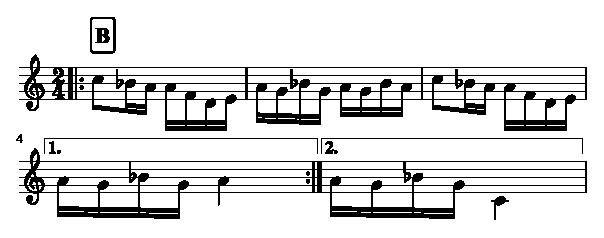
\includegraphics[width=\textwidth]{chapters/cap-musica-topicos/section-b-1.eps}}
	     \caption{Seção musical B.}
	     \label{fig:section-b}
     \end{figure}
A seção musical B está composta por B1 e B2; B1 está constituída pelos compassos 1,2,3 e 4; e B2 pelos compassos 1,2,3 e 5.

%%%%%%%%%%%%%%%%%%%%%%%%%%%%%%%%%%%%%%%%%%%%%%%%%%%%%%%%%%%%%%%%%%%%%%%%%%%%%%%%
\subsection{Criando a seção C}
\label{subsec:criandoc}
A seção musical C está composta por C1 e C2; 
C1 está constituída pelos compassos 1,2,3 e 4; e C2 pelos compassos 1,2,3 e 5.
A seção C foi criada para ser semelhante complementar da \hyperref[subsec:criandoa]{\textbf{seção B}},
com este propósito foi aplicada uma \hyperref[subsec:inversaovertical]{\textbf{inversão vertical}} em B,
ao redor da nota ``sol'', junto com uma transposição de +7 semitons.
Finalmente, a última nota de C1 e C2 foi modificada para que as cadencias continuem sendo (V-VI)  e (V-I),
respetivamente. 
A Figura \ref{fig:section-c} mostra a seção C.
     \begin{figure}[H]
	     \centering
	     \href{https://drive.google.com/file/d/1Z579dnspYxfRsBRGK-HfRwlppM2fr37L/view?usp=sharing}{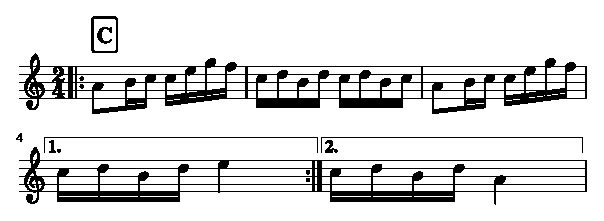
\includegraphics[width=\textwidth]{chapters/cap-musica-topicos/section-c-1.eps}}
	     \caption{Seção musical B.}
	     \label{fig:section-c}
     \end{figure}

%%%%%%%%%%%%%%%%%%%%%%%%%%%%%%%%%%%%%%%%%%%%%%%%%%%%%%%%%%%%%%%%%%%%%%%%%%%%%%%%
\subsection{Criando a introdução}
Para criar a seção de introdução, 
com dois \hyperref[subsec:compassobinario]{\textbf{compassos binários}} como mostrado na Figura \ref{fig:section-intro},
foi usado o ritmo do segundo compasso da \hyperref[subsec:criandoa]{\textbf{seção A}} 
junto com uma seleção de algumas notas usadas nessa seção. 
Isto foi feito assim para acostumar aos ouvintes à informação da melodia da seção A.
     \begin{figure}[H]
	     \centering
	     \href{https://drive.google.com/file/d/11yCuZzXDe-fD9OxCfYYR1-B3IfPG70cV/view?usp=sharing}{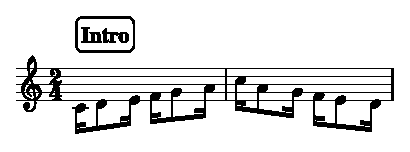
\includegraphics[width=0.7\textwidth]{chapters/cap-musica-topicos/section-intro-1.eps}}
	     \caption{Seção de introdução.}
	     \label{fig:section-intro}
     \end{figure}

%%%%%%%%%%%%%%%%%%%%%%%%%%%%%%%%%%%%%%%%%%%%%%%%%%%%%%%%%%%%%%%%%%%%%%%%%%%%%%%%
\subsection{Criando a coda}
A seção de coda está composta por dois \hyperref[subsec:compassobinario]{\textbf{compassos binários}}, 
como é mostrado na Figura \ref{fig:section-coda};
esta seção foi criada devido a que as seções 
\hyperref[subsec:criandoa]{\textbf{A}},
\hyperref[subsec:criandob]{\textbf{B}} e
\hyperref[subsec:criandoc]{\textbf{C}}
terminam num tempo fraco, dando uma sensação de não completitude ou suspense.
Assim a coda cumpre a função de criar uma transição suave ate um fim em tempo forte,
para gerar um final com sensação de completitude.
     \begin{figure}[H]
	     \centering
	     \href{https://drive.google.com/file/d/13WULHlz-Dfc6xnU0shYjoCc7OtJUWUVs/view?usp=sharing}{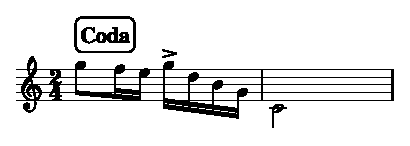
\includegraphics[width=0.7\textwidth]{chapters/cap-musica-topicos/section-coda-1.eps}}
	     \caption{Seção de coda.}
	     \label{fig:section-coda}
     \end{figure}

%%%%%%%%%%%%%%%%%%%%%%%%%%%%%%%%%%%%%%%%%%%%%%%%%%%%%%%%%%%%%%%%%%%%%%%%%%%%%%%%
\subsection{Estruturando as seções}

\begin{example}[Conversa rápida]
Podemos criar uma composição musical na \hyperref[subsec:formabinaria]{\textbf{forma binária}}, usando as seções 
\hyperref[subsec:criandoa]{\textbf{A}} e 
\hyperref[subsec:criandob]{\textbf{B}}.
Finalmente, foram agregadas também uma introdução e uma coda no inicio e final, respetivamente; 
como é mostrado na seguinte figura.
\begin{center}
	     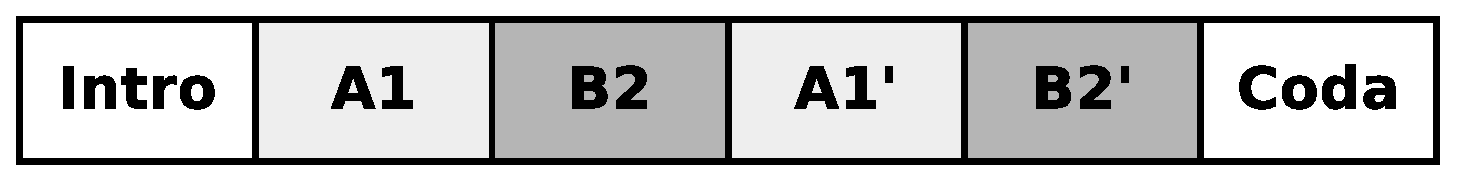
\includegraphics[width=0.70\textwidth]{chapters/cap-musica-topicos/section-cancao-block.eps}
\end{center}
A forma binária, pode ser interpretada seguindo as caraterísticas das melodias em cada seção, 
e correlacionando esta informação com as funções das 
\hyperref[subsec:partesmusica]{\textbf{partes da música}};
obtendo uma estrutura como:
\begin{center}
	     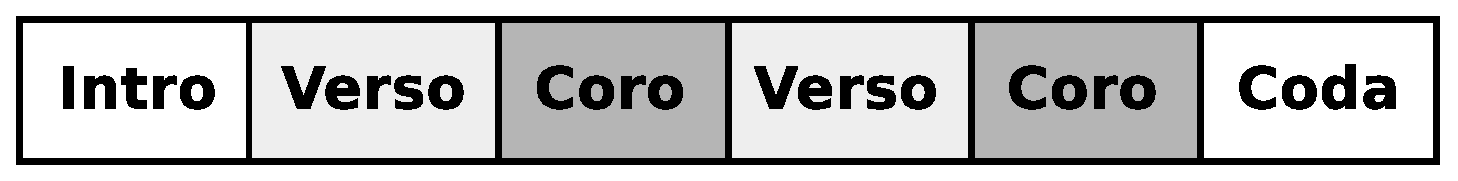
\includegraphics[width=0.70\textwidth]{chapters/cap-musica-topicos/section-cancao-block2.eps}
\end{center}
De modo que  A1 e A1' cumpram a função de versos  e, B2 e B2' a função de  coro.  \\
O resultado final pode ser visto na Figura \ref{fig:section-cancao};
esta composição está liberada baixo a 
\hyperref[ref:licensalivre]{\textbf{licença livre}}: 
\hyperref[subsec:CCBYSA]{\textbf{CC BY-SA}}.
\end{example}



\begin{example}[Conversa fina]
Podemos criar uma composição musical na \hyperref[subsec:formarondo]{\textbf{forma rondó}}, usando as seções 
\hyperref[subsec:criandoa]{\textbf{A}}, 
\hyperref[subsec:criandob]{\textbf{B}}, e
\hyperref[subsec:criandob]{\textbf{C}}.
Finalmente, foram agregadas também uma introdução e uma coda no inicio e final, respetivamente; 
como é mostrado na seguinte figura.
\begin{center}
	     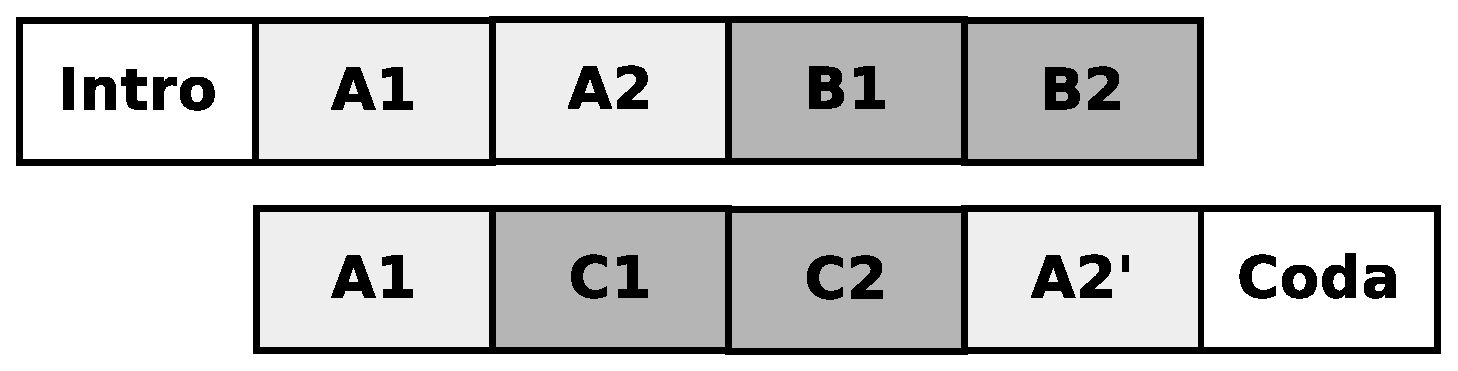
\includegraphics[width=0.70\textwidth]{chapters/cap-musica-topicos/section-choro-block.eps}
\end{center}
A forma rondó, pode ser interpretada seguindo as caraterísticas das melodias em cada seção, 
e correlacionando esta informação com as funções das 
\hyperref[subsec:partesmusica]{\textbf{partes da música}};
obtendo uma estrutura como: 
\begin{center}
	     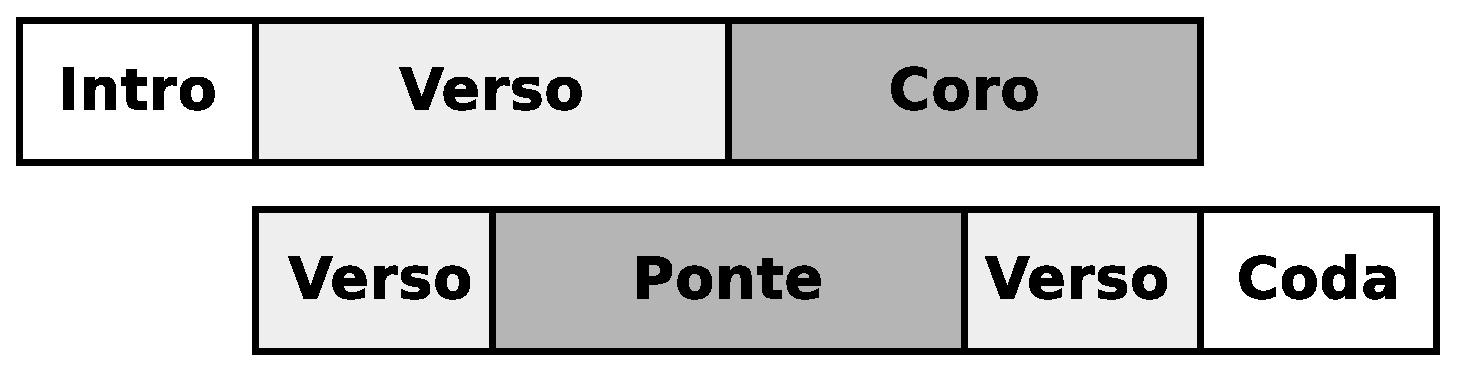
\includegraphics[width=0.70\textwidth]{chapters/cap-musica-topicos/section-choro-block2.eps}
\end{center}
%\{ Introdução,Verso, Coro, Verso, ponte, Verso, Coda\}.
De modo que  A, A1 e A2' cumpram a função de versos,  B a função de coro, e C a de ponte. \\
O resultado final pode ser visto na Figura \ref{fig:section-choro};
esta composição está liberada baixo a 
\hyperref[ref:licensalivre]{\textbf{licença livre}}:
\hyperref[subsec:CCBYSA]{\textbf{CC BY-SA}}.
\end{example}



\newpage
     \begin{figure}[!ht]
	     \centering
	     \href{https://drive.google.com/file/d/1RrfZT-o57iWbAx4Qks9vO_h6tBwVgNF7/view?usp=sharing}{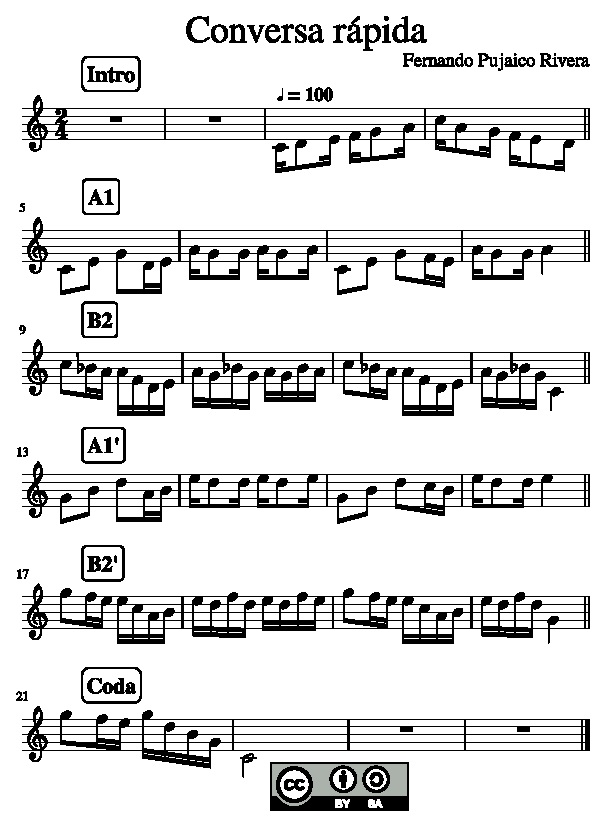
\includegraphics[width=1.0\textwidth]{chapters/cap-musica-topicos/section-cancao-1.eps}}
	     \caption{Música na forma binária.}
	     \label{fig:section-cancao}
     \end{figure}

\newpage
     \begin{figure}[!ht]
	     \centering
	     \href{https://drive.google.com/file/d/1eIO8uOb6IEr4pKfd2zZi1XfJvtqhbAPj/view?usp=sharing}{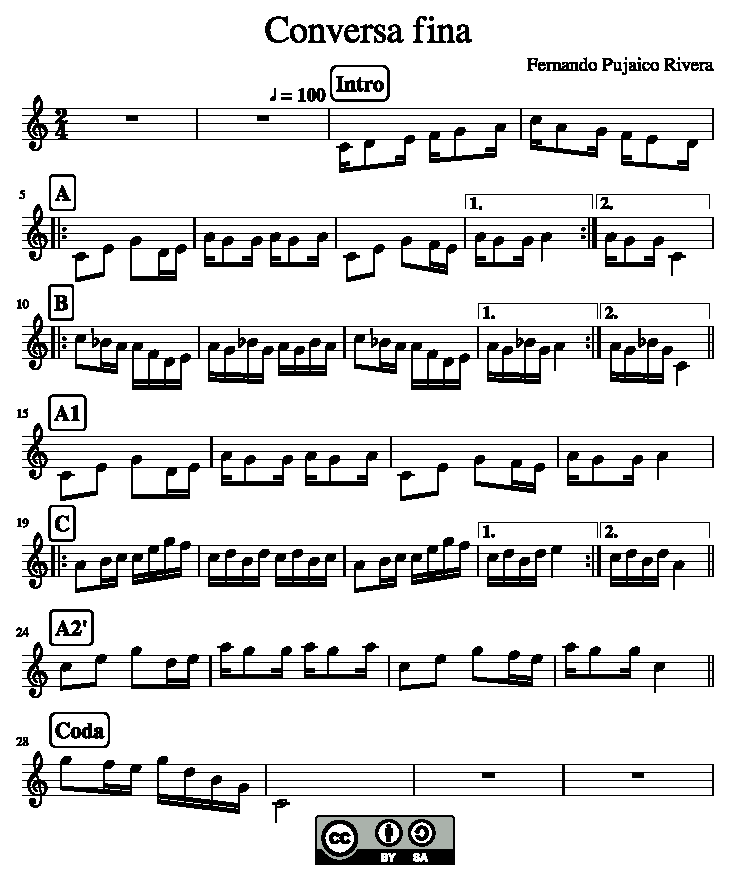
\includegraphics[width=1.0\textwidth]{chapters/cap-musica-topicos/section-choro-1.eps}}
	     \caption{Música na forma rondó.}
	     \label{fig:section-choro}
     \end{figure}

\newpage


